\documentclass[main.tex]{subfiles}
\newcommand\chapterlabel{equilibrium}
\setcounter{figurenewcounter}{0}


\begin{document}
\linenumbers
%\setcounter{chapter}{5}
  
\chapter[Chemical equilibrium]{Chemical equilibrium}
%\label{ch:atoms}


      \begin{marginfigure}
      \begin{tikzpicture} \node (a) at (0,0) {\includegraphics[width=4cm]{chapter18/figure1}} node[rotate=90, font=\tiny] at ([yshift=.5cm,xshift=.1cm]a.south east) {\textsuperscript{\textcopyright} PxFuel} ;
\end{tikzpicture}
\end{marginfigure}


\lettrine[lines=4]{\color{black!45}R}{eactions} rarely occur to completion. Once the products are formed they can follow a backward reaction to regenerate the reactants and at the same time, reactants regenerate produce products. Overall chemical reactions proceed until an equilibrium is reached. The equilibrium conditions determine how profitable a reaction can be as it describes how much of the products stay as products. This chapter covers the idea and basic principles of chemical equilibrium. We will describe the role of an equilibrium constant which gives insight into the mixtures of reactants and products in equilibrium. Also, we will discuss the different types of equilibrium constants in terms of molarity and pressure and the role of a reaction quotient giving insight into the direction in which a chemical reaction proceeds towards the equilibrium. Finally, we will cover  Le Ch\^{a}telier principle that describes once an equilibrium is altered, in which direction does a chemical reaction proceed to recover the equilibrium state.
 
\begin{marginfigure}%LEARNING GOALS BOX
\begin{mytcbox}{GOALS}
\begin{enumerate}[label=\protect\circled{\color{white}\arabic*}]
\item Formulate equilibrium constants
\item Interconvert $K_c$ and $K_p$
\item Apply Le Ch\^{a}telier
\item Interpret the magnitude of $K_c$
\item Carry simple equilibrium calculations
\end{enumerate}
\end{mytcbox}
\vspace{1cm}
\begin{tcolorbox}[enhanced,colback=red!5!white,colframe=black!50!red,boxrule=1pt,
  arc=0pt,outer arc=0pt,drop heavy lifted shadow]
\faGears\ 
\docenvdef{Discussion:} How can you make a reaction go faster? Give three possible answers. \end{tcolorbox}
\end{marginfigure}%LEARNING GOALS BOX

\section{Chemical Equilibrium and equilibrium constant}
This section covers basic ideas about chemical equilibrium. 
First, we will introduce the concept of the forward and reverse reaction. Next, we will define the idea of equilibrium, based on the speed of the forward and reverse reactions. Finally, we will show you how to interpret and calculate the numerical value of an equilibrium constant.

\sloppy

\begin{description}
\item[\docfilehook{Forward and reverse reactions}{Forward and reverse reactions}] In chemical reactions reactants form products. We call this the \emph{forward reaction}:
\begin{center}reactants $\ce{->}$ products \end{center}
However, once the products form they can also generate reactants through the \emph{reverse reaction}: 
\begin{center}reactants $\ce{<-}$ products\end{center}
\item[\docfilehook{Equilibrium}{Equilibrium}] In chemical reactions, both the forward and the reverse reaction happen synchronously, so that when products form they also generate reactants. However, both the reverse and forwards reactions have different speeds. In the beginning, the forward reaction proceeds at a faster pace than the reverse so that the reaction advances. Once products form, the reverse reaction will start speeding. A reaction reaches \emph{chemical equilibrium} when both the forward and reverse reactions proceed at the same speed. 
Chemical reactions normally are written down with a double arrow that indicates equilibrium:
\begin{center}reactants $\ce{<=>}$ products\end{center}
For example, the chemical process that forms ammonia from nitrogen and hydrogen can proceed using the forward and reverse reaction
\begin{center}\ce{3H2 + N2 <=>[$\textcolor{red}{\text{Forward Reaction}}$][$\textcolor{blue}{\text{Reverse Reaction}}$] 2NH3}\end{center}
\begin{marginfigure}[-0cm]%%%%%%%% MARGIN FIGURE
\begin{tikzpicture}\node[anchor=south west,inner sep=0] (image) at (0,0,0) {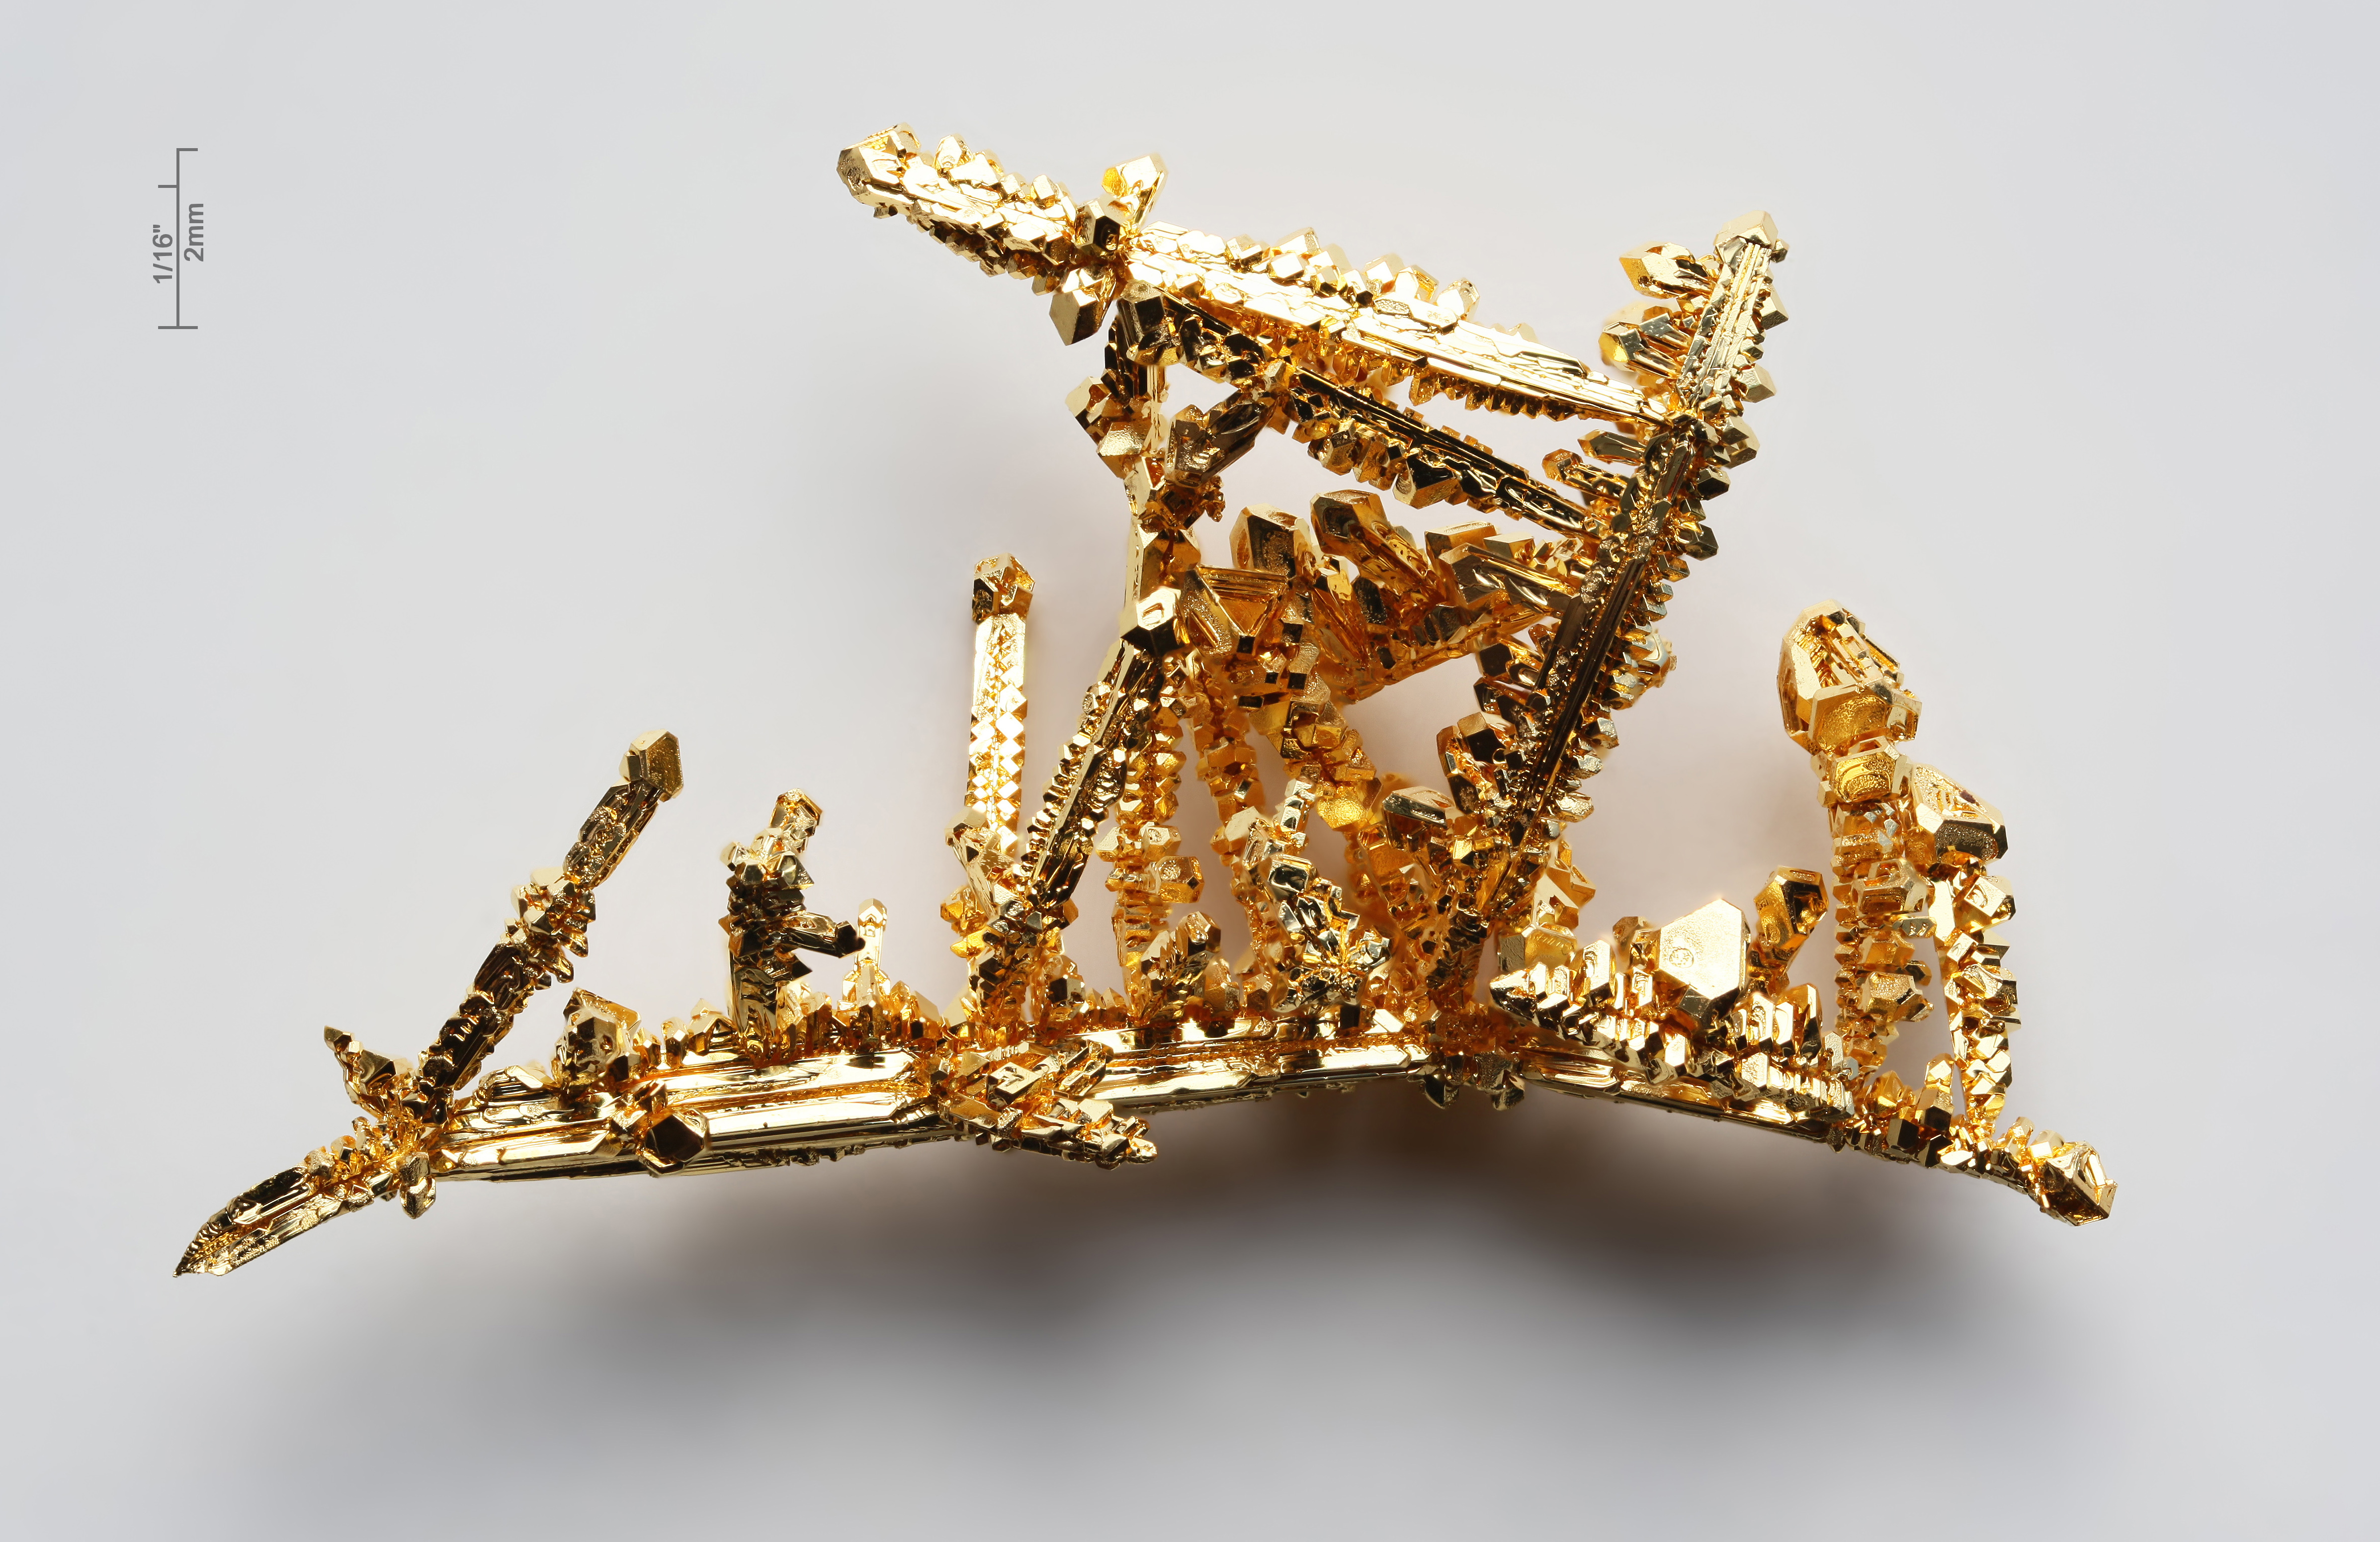
\includegraphics[width=1\columnwidth]{chapter18/figure6}};
 \node [font=\Large ] at (1cm,6cm)  {
 \begin{tabular}{c}
Reverse  \\
reaction  \\
\end{tabular} };
 \node [font=\Large ] at (1cm,12cm)  {
 \begin{tabular}{c}
Forward  \\
reaction  \\
\end{tabular} };
\end{tikzpicture}
\caption{The forward reaction goes from reactants to products whereas the reverse reaction goes from products to reactants. }
\end{marginfigure}%%%%%%% MARGIN FIGURE
\item[\docfilehook{Equilibrium and concentration}{Equilibrium and concentration}] 
It is just a matter of time that a reaction reaches equilibrium. Initially, the forward process normally proceeds at high speed as products start to form. This is because initially there is an abundance of reactants. Once the products start to accumulate the forward process will start happening. This is because at that point there is an increasing amount of product molecules that can go back to reactants. Eventually, the forward and reverse rates become equal as the reaction reaches equilibrium. When the equilibrium has been reached, reactants and products have very specific concentrations. At the same time, a reaction in equilibrium contains a mixture of reactants and products.

\begin{example} %%%%%%%%%%%%%%%%%%%%%%%% EXAMPLE BOX
Write down the forward and reverse reactions for:
\begin{center}\ce{CH4(g) + 2O2(g) <=> CO2(g) + 2H2O(g)}\end{center}
\textlcsc{ \textcolor{dgreen}{\Large \textbf{Solution}} }\\
(a) The forward reaction is \ce{CH4(g) + 2O2(g) -> CO2(g) + 2H2O(g)} and the reverse \ce{CH4(g) + 2O2(g) <- CO2(g) + 2H2O(g)}
\\
\faDiamond\ \textlcsc{ \textcolor{dgreen}{\Large \textbf{Study Check}} }\\
Write down the forward and reverse reactions for the reaction: \begin{center}\ce{CO(g) + O2(g) <=> CO2(g) }\end{center}

\flushright  {\small Answer: \ce{CO(g) + O2(g) -> CO2(g)} and \ce{CO(g) + O2(g) <- CO2(g)}}
\end{example}%%%%%%%%%%%%%%%%%%%%%%%% EXAMPLE BOX
%\end{description}
%
%\newpage
%\section{{The equilibrium constant}}
%Reactions in equilibrium are characterized buy an equilibrium constant. This next section will show you how to interpret and calculate the value of the equilibrium constant of a reaction.
%\sloppy
%
%\begin{description}

\item[\docfilehook{Equilibrium mixtures}{Equilibrium mixtures}] Imagine you start a chemical reaction. Initially, products will form and reactants will disappear. At equilibrium, you will have a mixture of reactants and products with the forward and reverse processes happening at the same rate. The question is: an equilibrium mixture would contain more reactants or perhaps more products? The equilibrium constant helps predict just that.
\item[\docfilehook{The equilibrium constant of a reaction}{The equilibrium constant of a reaction}] The equilibrium constant associated with a reaction $K_c$ indicates whether there is an abundance of reactants or products at equilibrium. Each reaction has one $K_c$ value that depends only on temperature and the subscript $_c$ represents concentration. On one hand, if $K_c$ is larger than one there will be a larger concentration of products than reactants in the equilibrium mixture. On the other hand, if  $K_c$ is smaller than one there will be a larger concentration of reactants than products in the equilibrium mixture. If  $K_c$ is close to one then both reactants and products will have the same concentration in the equilibrium mixture. 
 \begin{center}\begin{tikzpicture}[colorbar arrow/.style={
  shape=double arrow,
  double arrow head extend=0.125cm, 
  shape border rotate=0, 
  minimum height=10cm,minimum width=2cm,
  shading=#1 
}]

\node [colorbar arrow=shading1] (thickarrow) at (0,0) {};
  \node[font=\large]  at (-3cm,0cm) {Mostly Reactants};   \node[font=\large]  at (3cm,0cm) {Mostly Products}; 
\node[font=\large, below = 3mm of thickarrow]  at (-3cm,-1cm) { $K_{c}<1$};    \node[font=\large, below = 3mm of thickarrow]  at (0cm,-1cm) {$K_{c}\simeq 1$};  \node[font=\large, below = 3mm of thickarrow]  at (3cm,-1cm) {$K_{c}>1$}; 
\end{tikzpicture}  \end{center}

In terms of units, equilibrium constants are unitless numbers. In other words, they have no unit and they are simply expressed as a number.



\begin{example} %%%%%%%%%%%%%%%%%%%%%%%% EXAMPLE BOX
The value of $K_{c}$ for the following reaction at 300K is $4\times 10^{31}$. Indicate whether the equilibrium mixture will contain mostly reactants, mostly products of both.
\begin{center}\ce{Cl2_{(g)} + H2_{(g)} <=> 2HCl_{(g)}}\end{center}
\textlcsc{ \textcolor{dgreen}{\Large \textbf{Solution}} }\\
As $K_{c}$ is larger than one, an equilibrium mixture of \ce{Cl2},  \ce{H2} and  \ce{HCl} will contain mainly products, that is will be mainly made of \ce{HCl}.
\\
\faDiamond\ \textlcsc{ \textcolor{dgreen}{\Large \textbf{Study Check}} }\\
The value of $K_{c}$ for \ce{F2(g) <=> 2F(g)} at 500K is $7\times 10^{-13}$. Indicate whether the equilibrium mixture will contain mostly reactants, mostly products of both.
\\
\flushright  {\small Answer: mostly reactants. }
\end{example}%%%%%%%%%%%%%%%%%%%%%%%% EXAMPLE BOX
\begin{marginfigure}[-0cm]%%%%%%%% MARGIN FIGURE
\begin{tikzpicture}\node[anchor=south west,inner sep=0] (image) at (0,0,0) {\includegraphics[width=1\columnwidth]{chapter18/figure7}};
 \node [font=\Large ] at (4cm,5cm)  {
 \begin{tabular}{c}
$K_{c}<1$   \\
\end{tabular} };
 \node [font=\Large ] at (4cm,10cm)  {
 \begin{tabular}{c}
$ K_{c}=1$  \\
\end{tabular} };
 \node [font=\Large ] at (4cm,16cm)  {
 \begin{tabular}{c}
$K_{c}>1$  \\
\end{tabular} };
\end{tikzpicture}
\caption{The equilibrium constant tells you whether there is more products or reactants in an equilibrium mixture.  }
\end{marginfigure}%%%%%%% MARGIN FIGURE



\item[\docfilehook{Equilibrium constant expression}{Equilibrium constant expression}] Let's consider a general equilibrium reaction in which $A$ and $B$ react to form $C$ and $D$
\begin{center}\ce{$\underbrace{\textcolor{red}{\ce{aA + bB}}}_{\textrm{Reactants}}$ <=> $\underbrace{\textcolor{blue}{\ce{cC + dD}}}_{\textrm{Products}}$}
\end{center}
The stoichiometric coefficients of the reaction are: $a$, $b$, $c$ and $d$. The expression for the equilibrium constant depends only on the concentration of the reactants and products. In order to refer to concentration we will user square brackets. For example $\big[ A \big]$ means the concentration of $A$. Hence, the expression of the equilibrium constant will be:

\begin{equation}
\boxed{  K_{c}=\frac{\big[\text{Products}\big]}{\big[\text{Reactants}\big]}=\frac{\big[ C \big]^c \cdot \big[ D \big]^d} {\big[ A \big]^a \cdot \big[ B \big]^b} } \quad \textcolor{blue}{\text{Equilibrium constant}}\label{\chapterlabel:equation1}
\end{equation}
%\resizeableyellownote{2.5}{1}{Add  Formula \textcolor{blue}{\ref{formula1:1}} to your flashcard.}

Let us break down the expression of $K_c$. On top of the fraction we have the equilibrium concentration of the products to the power of its coefficients. For example $\big[ C \big]^c$ means the equilibrium concentration of $C$ to the power of the coefficient $c$. On the bottom of the fraction we have  the concentration of the reactants to the power of its coefficients. All concentrations in $K_{c}$ are timed.
 \begin{center}\begin{tikzpicture}[> = stealth']
  \node[font=\Large] (alta) {$\big[ C \big]^c \cdot \big[ D \big]^d$}; 
  \node[font=\Large, below = 3mm of alta] (baja) {$\big[ A \big]^a \cdot \big[ B \big]^b$};
\node [font=\Large] at ([shift={(3mm:-6mm)}]alta.south west) {$K_{c}=$};
  \draw[thick, <-] (alta) --++(40:1cm) node[right, text width=5cm, align=left]{\small{product concentration }};
  \draw[thick, <-] (baja.east) --++(-60:1cm) node[right, text width=5cm, align=left]{\small{reactant coefficient }};
  \draw[thick] ([yshift=-1.5mm]alta.south west) --  ([yshift=-1.5mm]alta.south east);
 \end{tikzpicture}\end{center}
Let's focus on the reaction below:
\begin{center}\ce{CH4_{(g)} + 2O2_{(g)} <=> CO2_{(g)} + 2H2O_{(g)}}\end{center}
The expression of the equilibrium constant would be:
\begin{equation*}
  K_{c}=\frac{\big[ \ce{CO2} \big] \cdot \big[ \ce{H2O} \big]^2} {\big[ \ce{CH4} \big] \cdot \big[ \ce{O2} \big]^2} 
\end{equation*}


\item[\docfilehook{Equilibrium involving solids, liquids and solutions}{Equilibrium involving solids, liquids and solutions}] 
Let us analyze an example of a reaction involving solids or liquids:
\begin{center}\ce{CaCO3 * H2O_{(s)} <=> CaO_{(s)} + CO2_{(g)} + H2O_{(l)}}\end{center}
Solids and liquids have no concentration and hence they should not included in the expression of $K_c$. For the example above:
\begin{equation*}
  K_{c}=\big[ \ce{CO2} \big]
\end{equation*}
Differently for reaction involving aqueous solutions, for example:
\\\ce{HCl_{(Aq)} <=> H^+_{(Aq)} + Cl^-_{(Aq)}}\hfill $K_{c}=\frac{[\ce{H^+}]\cdot [\ce{Cl^-}]}{[\ce{HCl}]}$\\
Overall, remember that in the expression of $K_c$ you can only include gases (g) or aqueous solutions (aq) as you can ignore solids and liquids without a well-defined concentration.

\begin{example} %%%%%%%%%%%%%%%%%%%%%%%% EXAMPLE BOX
Write down the expression of $K_c$ for the following reactions:\\
(a) \ce{2NO2_{(g)} <=> N2O4_{(g)}}\\
(b) \ce{C3H8_{(g)} + 5O2_{(g)} <=>  4H2O_{(g)} + 3CO2_{(g)}}\\
(c) \ce{Zn_{(s)} + 2 HCl_{(Aq)} <=> ZnCl2_{(Aq)} + H2_{(g)}}
\\
\textlcsc{ \textcolor{dgreen}{\Large \textbf{Solution}} }\\
Remember you can only include gas and aqueous solution in the expression of $K_c$. For the first example
\begin{equation*} K_{c}=\frac{\big[ \ce{N2O4} \big]} {\big[ \ce{NO2} \big]^2 } \end{equation*}
For the second example,
 \begin{equation*} K_{c}=\frac{\big[ \ce{H2O} \big]^4 \cdot \big[ \ce{CO2} \big]^3} {\big[ \ce{C3H8} \big] \cdot \big[ \ce{O2} \big]^5} \end{equation*}
For the last example:
\begin{equation*}  K_{c}=\frac{\big[ \ce{ZnCl2} \big] \cdot \big[ \ce{H2} \big]} {\big[ \ce{HCl} \big]^2}\end{equation*} 
\\
\faDiamond\ \textlcsc{ \textcolor{dgreen}{\Large \textbf{Study Check}} }\\
Write down the expression of $K_c$ for the following reaction:\\
 \ce{Pb^{2+}_{(Aq)} + 2I^{-}_{(Aq)} <=> PbI2(s)}.
\flushright  {\small Answer: $\frac{1} {\big[ \ce{Pb^{2+}} \big] \cdot \big[ \ce{I^-} \big]^2 }$ }
\end{example}%%%%%%%%%%%%%%%%%%%%%%%% EXAMPLE BOX


\item[\docfilehook{Equilibrium constant in terms of pressures}{Equilibrium constant in terms of pressures}] 
The equilibrium constant $K_{c}$ is the ratio of the concentration of products and reactants. As concentration is related to pressure--remember the chapter about gases--we can also express an equilibrium constant in terms of pressures, we call this $K_{p}$.
\begin{equation}
\boxed{  K_{p}=\frac{P_{\text{Products}}}{P_{\text{Reactants}}}=\frac{P_{C}^c \cdot P_{D}^d} {P_{A}^a \cdot P_{B}^b} } \quad \textcolor{blue}{\text{Equilibrium constant}}
\label{\chapterlabel:equation2}
\end{equation}
Let's focus on an example. Think about the reaction below that involved just gases:
\begin{center}\ce{CH4_{(g)} + 2O2_{(g)} <=> CO2_{(g)} + 2H2O_{(g)}}\end{center}
The expression of the equilibrium constant would be:
\begin{equation*}
  K_{p}=\frac{P_{\ce{CO2}} \cdot P_{\ce{H2O}}^2} {P_{\ce{CH4}} \cdot P_{\ce{O2}}^2} 
\end{equation*}
$K_{p}$ values larger than one imply that in the mixture the pressure of products is larger than the pressure of reactants and the opposite is true for values smaller than one.
\item[\docfilehook{Relating $K_{c}$ and $K_{p}$}{Relating $K_{c}$ and $K_{p}$}] 
The values of $K_{c}$ and $K_{p}$ are related by the following formula:
\begin{equation}
\boxed{  K_p=K_c (RT)^{\Delta n}}
\label{\chapterlabel:equation3}
\end{equation}
where:
\begin{where}
 \item $K_p$   is the equilibrium constant in terms of pressure
 \item $K_c$   is the equilibrium constant in terms of concentration
 \item $R$  is the constant of the gases in pressure units (0.083 atmL/molK)
  \item $T$  is the absolute temperature (in Kelvins)
    \item $\Delta n$  is the change of stoichiometry of the reaction
\end{where}
Let us analyze the role of $\Delta n$ for the reaction:
\begin{center}\ce{C3H8 + 5O2 <=> 4H2O + 3CO2}\end{center}  
$\Delta n$ represents the number of molecules of products with respect to the number of molecules of reactants: 7-6=1. For this reaction, we have that $K_p=K_c (RT)$. However, the power on the relationship will depend on the stoichiometry of the reaction. At the same time, the relationship between both constant depends on the tempertaure.
\begin{example} %%%%%%%%%%%%%%%%%%%%%%%% EXAMPLE BOX
For the following reaction
\begin{center}\ce{2NH3_{(g)}  <=> N2_{(g)}	+ 3H2_{(g)}		}\end{center}
The value of $K_c$ at 300K is 17. Calculate the value of $K_p$ at the same temperature.
\textlcsc{ \textcolor{dgreen}{\Large \textbf{Solution}} }\\
First we will write down the expression of both equilibrium constants:
\begin{center}$K_{c}=\frac{	\big[ \ce{NH3} \big]^2 			} {	\big[ \ce{N2} \big]\cdot \big[ \ce{H2} \big]^3	}$\hspace{1cm}
$K_{p}=\frac{	P_{\ce{NH3}}^2  		} {P_{\ce{N2}}	\cdot P_{\ce{H2}}^3		}$\end{center}
We will also calculate $\Delta n$ in order to establish the relationship between both constants:
\[\Delta n=1+3-2=2\]
We have that:
\[K_p=K_c (RT)^{\Delta n}=K_c (RT)^2\]
Given than $K_c$ at 300K is 17:
\[K_p=K_c (RT)^{\Delta n}=17 (0.082\cdot 300)^2=10287\]
In equilibrium, the pressure of products will be larger than the pressure of reactants.\\
\faDiamond\ \textlcsc{ \textcolor{dgreen}{\Large \textbf{Study Check}} }\\
For the following reaction
\begin{center}\ce{	SO2Cl2_{(g)} <=> SO2_{(g)} + Cl2 _{(g)}		}\end{center}
The value of $K_p$ at 300K is 0.05. Calculate the value of $K_c$ at the same temperature.\\
\flushright  {\small Answer: $	2]times 10^{-3}$ }
\end{example}%%%%%%%%%%%%%%%%%%%%%%%% EXAMPLE BOX






\end{description}




\section{ {Using equilibrium constants}}
We saw that the equilibrium constant of a reaction tells you whether there are more reactants or products in an equilibrium mixture. At the same time, one can use $K_c$ to quantitatively calculate the value of the equilibrium concentration of reactants and products. This section will explain how to do this.
\sloppy
\begin{description}
\item[\docfilehook{Solving from $K_c$}{Solving from $K_c$}] Let's analyze the reaction of hydrogen (\ce{H2}) and iodine (\ce{I2}) to produce hydrogen iodide (\ce{HI}):
\begin{center}\ce{H2(g) + I2(g) <=> 2HI(g)}\end{center}
The equilibrium constant at 300K is $3\cdot 10^{-1}$. Analyzing a reaction mixture we find that the concentration of \ce{H2} is 1M and the concentration of \ce{I2} is 2M. We want to calculate how much \ce{HI} do we have in the mixture. As the concentrations of reactants and products are linked together through $K_c$ we can certainly solve for $\big[ \ce{HI} \big]$. The expression for $K_c$ is:
\begin{equation*}  K_{c}=\frac{\big[ \ce{HI} \big]^2 } {\big[ \ce{H2} \big] \cdot \big[ \ce{I2} \big]}\end{equation*} 
and we know that $\big[ \ce{H2} \big]=1M$ and $\big[ \ce{I2} \big]=2M$. Plugging the values in the expression of $K_c$, and given the numerical value of $K_c$ we have:
\begin{equation*} 3\cdot 10^{-1}=\frac{\big[ \ce{HI} \big]^2 } {1 \cdot 2^2}\end{equation*} 
Solving for $\big[ \ce{HI} \big]$ we have 
\begin{equation*} \big[ \ce{HI} \big]^2=1.2     \end{equation*} 
To solve for $\big[ \ce{HI} \big]$ we have to use an square root:
\begin{equation*} \big[ \ce{HI} \big]=\sqrt[2]{1.2}=1.09M     \end{equation*} 
\marginnote{\faBicycle\ Remember: the square root  key in your calculator looks like \keystroke{\large $\sqrt{}$}.}
\begin{example} %%%%%%%%%%%%%%%%%%%%%%%% EXAMPLE BOX
The value of the equilibrium constant for the reaction 
 \begin{equation*} \ce{3H2(g) + N2(g) <=>  2NH3(g)} \end{equation*}
 is $3\cdot 10^{8}$ at 300K. An analysis of an equilibrium mixture gave a concentration of nitrogen and ammonia of 2M, respectively. Calculate the equilibrium concentration of hydrogen at 300K.
 \\
\textlcsc{ \textcolor{dgreen}{\Large \textbf{Solution}} }\\
The value of the equilibrium constant for the formation of ammonia is: 
 \begin{equation*} K_{c}=\frac{\big[ \ce{NH3} \big]^2 }{\big[ \ce{H2} \big]^3 \cdot \big[ \ce{N2} \big]}  \end{equation*}
We know $\big[ \ce{NH3} \big]$ and $\big[ \ce{N2} \big]$ and both values are 2M, and we also know $ K_{c}=3\cdot 10^{8}$. Plugging these values into the previous equations we obtain:
 \begin{equation*}3\cdot 10^{8}=\frac{2^2 } {\big[ \ce{H2} \big]^3 \cdot 2} \end{equation*}
we can solve for $\big[ \ce{H2} \big]$:
 \begin{equation*}\big[ \ce{H2} \big]^3= 6.6\cdot 10^{-9}   \end{equation*}
In order to obtain $\big[ \ce{H2} \big]$ we need a a cubic root:
 \begin{equation*}\big[ \ce{H2} \big]= \sqrt[3]{6.6\cdot 10^{-9}} =1.9\cdot 10^{-3}M  \end{equation*}
\\
\faDiamond\ \textlcsc{ \textcolor{dgreen}{\Large \textbf{Study Check}} }\\
The value of the equilibrium constant for the reaction \begin{center}\ce{C3H8 + 5O2 <=> 4H2O + 3CO2}\end{center}  is $500$ at a given temperature. An analysis of an equilibrium mixture gave a concentration of water, carbon dioxide and \ce{C3H8} of 1M. Calculate the equilibrium concentration of oxygen at that temperature.\\
 \flushright  {\small Answer: $\big[ \ce{O2} \big]=0.43M$ }
\end{example}%%%%%%%%%%%%%%%%%%%%%%%% EXAMPLE BOX
\marginnote{\faBicycle\ Remember: to solve $x^5=100$ you need \keystroke{ $\sqrt[5]{}$}. You can solve this by typing: 100\keystroke{\^}\keystroke{ $(1/5)$} and the answer is 2.51.}

\end{description}
 



\section{ Concentration or pressure ratio}
In a chemical reaction, if we prepare a mixture of reactants they will generate products. At equilibrium reactants and products exist at a very specific ratio given by the equilibrium constant. 
What if we would prepare a mixture containing both reactants and products? Given that both reactants and products are related by an equilibrium, how would the concentrations change?
In other words, would the reaction proceed towards the right producing products or the left producing reactants? This section introduces the use of a concentration (or pressure) ratio that helps predicts the direction in which a mixture of reactants and products will proceed towards the equilibrium.
\sloppy
\begin{description}
\item[\docfilehook{Definition of concentration ratio	}{Definition of concentration ratio}] 
Equilibrium constant are ratios of equilibrium concentration or pressure of products over reactants measured after the system has reacted for an infinite time.
Concentration ratio $Q_c$ are ratios of concentration of products over reactants away from the equilibrium. In another words, they represent the reaction away from the equilibrium.
\begin{equation}
\boxed{  Q_{c}=\frac{\big[\text{Products}\big]_{noneq}}{\big[\text{Reactants}\big]_{noneq}}=\frac{\big[ C \big]_{noneq}^c \cdot \big[ D \big]_{noneq}^d} {\big[ A \big]_{noneq}^a \cdot \big[ B \big]_{noneq}^b} } \quad \textcolor{blue}{\text{concentration ratio}}\label{\chapterlabel:equation4}
\end{equation}

\item[\docfilehook{Use of concentration ratios	}{Use of concentration ratios	}] 
Concentration ratios helps predict whether a reaction will proceed towards the left or towards the right when we start with a mixture of reactants and products away from equilibrium.
 \begin{center}\begin{tikzpicture}[colorbar arrow/.style={
  shape=double arrow,
  double arrow head extend=0.125cm, 
  shape border rotate=0, 
  minimum height=10cm,minimum width=2cm,
  shading=#1 
}]

\node [colorbar arrow=shading1] (thickarrow) at (0,0) {};
  \node[font=\large]  at (-3cm,0cm) {$Q_c<K_c$};   \node[font=\tiny, rotate=90]  at (0cm,0cm) {Equilibrium}; \node[font=\large]  at (3cm,0cm) {$Q_c>K_c$}; 
  
%\node[font=\large, below = 3mm of thickarrow]  at (-3cm,-1cm) { $K_{c}<1$}; 
\draw[ultra thick, ->]  (-3cm,-1cm) --+(1cm,0cm) ; 
   \node[font=\large, below = 3mm of thickarrow, shift={(0cm,.5cm)}]  at (0cm,-1cm) {$K_c$};  
\draw[ultra thick, ->]  (3cm,-1cm) --+(-1cm,0cm) ; 
\end{tikzpicture}  \end{center}
If $Q_c$ is larger than $K_c$ the reaction will proceed towards the left producing reactants. On the other hand, if $Q_c$ is smaller than $K_c$ the reaction will proceed towards the right producing products. If $Q_c$ equals to $K_c$ then the reaction is in equilibrium.

\begin{example} %%%%%%%%%%%%%%%%%%%%%%%% EXAMPLE BOX
In two different experiments, we prepare mixtures of four chemicals interconnected by the following equilibrium:
\begin{center}\ce{CO_{(g)} + H2O_{(g)}	<=> CO2_{(g)}	+ H2_{(g)}}\hfill $K_c =0.48$\end{center}
Indicate if any of the mixtures is in equilibrium. If it is not, indicate whether the reaction will evolve towards the left or the right to reach equilibrium.

\begin{center}\begin{tabular}[t]{   ccc    }
\toprule
Experiment&			1		&	2		 \\
\midrule

$[\ce{CO2}]$&			0.0040	&	0.037	 \\
$[\ce{H2}]$&			0.0040	&	0.046	 \\
$[\ce{CO}]$&			0.0203	&	0.011	 \\
$[\ce{H2O}]$&			0.0203	&	0.0011	 \\
\bottomrule
\end{tabular}\end{center}
 
\textlcsc{ \textcolor{dgreen}{\Large \textbf{Solution}} }\\
We will compute the concentration ratio for each experiment and compare the value with $k_c$. If $Q_c$ is larger than $k_c$ the reaction will proceed to the left whereas if $Q_c$ is smaller than $k_c$ the reaction will proceed to the right.
\begin{center}\begin{tabular}[t]{   ccc    }
\toprule
Experiment&			1		&	2		 \\
\midrule
$[\ce{CO2}]$&			0.0040	&	0.037	 \\
$[\ce{H2}]$&			0.0040	&	0.046	 \\
$[\ce{CO}]$&			0.0203	&	0.011	 \\
$[\ce{H2O}]$&			0.0203	&	0.0011	 \\
$Q_c$&			$3.8\times 10^{-4}$	&	140	 \\
\bottomrule
\end{tabular}\end{center}
None of the mixtures are in equilibrium as $Q_c$ differs from $k_c$. In the first experiment the reaction will proceed to the right and in the second experiment the reaction will proceed to the left.
\\
\faDiamond\ \textlcsc{ \textcolor{dgreen}{\Large \textbf{Study Check}} }\\
We prepare mixtures of four chemicals in an experiment. These chemicals are interconnected by the following equilibrium:
\begin{center}\ce{CO_{(g)} + H2O_{(g)}	<=> CO2_{(g)}	+ H2_{(g)}}\hfill $K_c =0.48$\end{center}
Indicate if the mixture is in equilibrium. If it is not, indicate whether the reaction will evolve towards the left or the right to reach equilibrium.\begin{center}\begin{tabular}[t]{   cc     }
\toprule
Experiment&			1		 		 \\
\midrule
$[\ce{CO2}]$&			0.0015	 	 \\
$[\ce{H2}]$&			0.0076	 	 \\
$[\ce{CO}]$&			0.0094	 	 \\
$[\ce{H2O}]$&			0.0025	 	 \\
\bottomrule
\end{tabular}\end{center}
 \flushright  {\small Answer: to the right}
\end{example}%%%%%%%%%%%%%%%%%%%%%%%% EXAMPLE BOX








\end{description}

\begin{marginfigure}[-10cm]%%%%%%%% MARGIN FIGURE
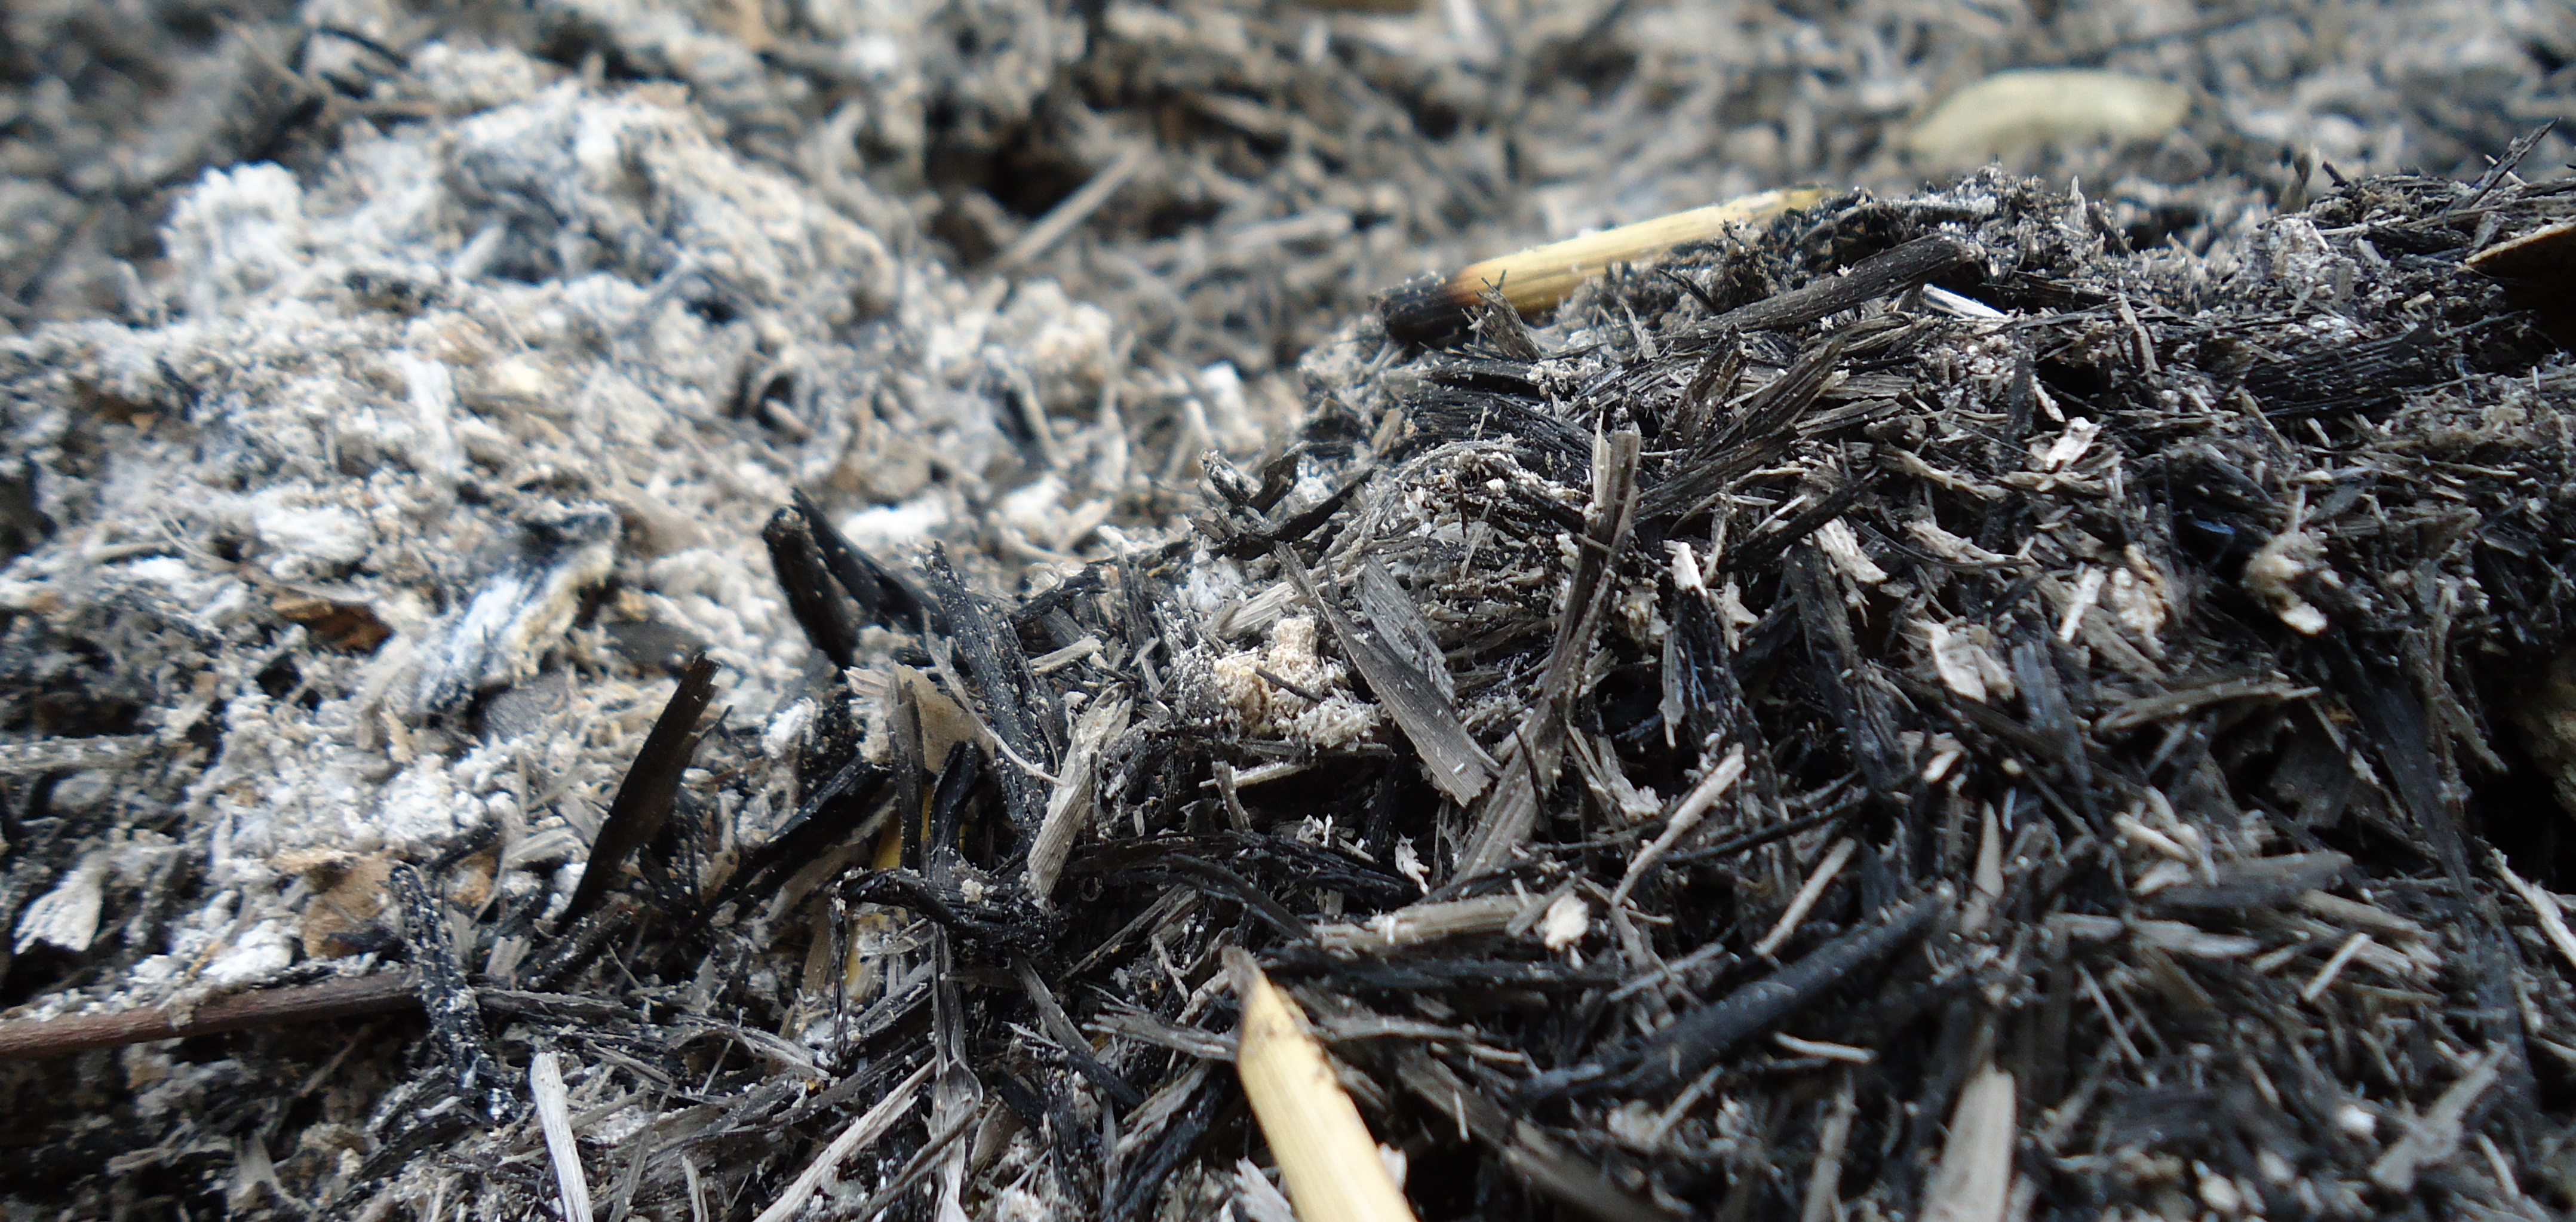
\includegraphics{chapter18/figure8}
\caption{ Henry Louis Le Ch\^{a}telier was a french chemist who devised a principle used by chemists to predict the effect a changing condition has on a system in chemical equilibrium. }
\end{marginfigure}%%%%%%% MARGIN FIGURE
\section{ {Le Ch\^{a}telier principle}}
At this point, we have covered the idea of equilibrium and we have seen that the forward and reverse reactions have the same rate at equilibrium. Now, what happens if you alter this equilibrium? Le Ch\^{a}telier principle claims a reaction will go back to its original equilibrium state by shifting left or right.
\sloppy
\begin{description}
\item[\docfilehook{Le Ch\^{a}telier principle}{Le Ch\^{a}telier principle}] 
When a reaction is in equilibrium the forward and reverse reactions proceed at the same speed. Also in an equilibrium state, the concentrations of reactants and products have very specific values. Imagine that you create stress conditions by adding reactants or products or even changing the temperature. This stress will have an impact on the equilibrium and the reaction eventually will reach a new state of equilibrium by somehow counteracting this stress.
 Le Ch\^{a}telier principle says that when a stress is placed in a reaction (adding or removing reactant or products, increasing decreasing temperature) the equilibrium will be shifted in the direction that relieves that stress. 
 
 \begin{marginfigure}[-6cm]%%%%%%%% MARGIN FIGURE
\begin{tikzpicture}\node[anchor=south west,inner sep=0] (image) at (0,0,0) {\includegraphics[width=1\columnwidth]{chapter18/figure13}};
 \node [font=\small ] at (3cm,12cm)  {
 \begin{tabular}{c}
Adding reactants shifts \\
 the equilibrium to the right \\
\end{tabular} };
 \node [font=\small ] at (2cm,7.5cm)  {
 \begin{tabular}{c}
Removing reactants shifts \\
 the equilibrium to the left \\
 \end{tabular} };
 \node [font=\small ] at (3cm,3.7cm)  {
 \begin{tabular}{c}
Adding products shifts \\
 the equilibrium to the left \\
 \end{tabular} };
  \node [font=\small ] at (2.5cm,-0.5cm)  {
 \begin{tabular}{c}
Warming an exothermic reaction \\
shifts the equilibrium to the left \\
 \end{tabular} };
\end{tikzpicture}
\caption{Le Ch\^{a}telier principle helps predicts the outcome of altering an equilibrium mixture.}
\end{marginfigure}%%%%%%% MARGIN FIGURE
 
 \item[\docfilehook{Change in concentration}{Change in concentration}] Let us consider the following equilibrium:
 \begin{equation*} \ce{CO2(g) + H2(g) <=> CO(g) + H2O(g)} \end{equation*}
$K_c$ for this reaction equals to one at 1200K. This means that the concentration of reactants and products are the same. We can represent this by means of this balance or seesaw
\begin{center}\tikzset{
  pivot/.style={
    draw, 
    regular polygon, 
    regular polygon sides = 3, 
    fill = red, 
    node distance = 1cm, 
    minimum height = 2em,
    at = {(0,0)}
  }
}
\begin{tikzpicture}
  \node [pivot] (a) {};\node [font=\tiny ]  {\ce{<=>}};
  \begin{scope}[rotate around={0:(a.corner 1)}]
   \draw (a.corner 1) -| ++(-3cm,5mm) node[transform shape,above] (t1) {\ce{CO2(g) + H2(g)}};
   \draw (a.corner 1) -| ++(3cm,5mm) node[transform shape,above] (t2) {\ce{CO(g) + H2O(g)}};
   \draw (t1.south east) -- (t1.south west);
   \draw (t2.south east) -- (t2.south west);
  \end{scope}
\end{tikzpicture}\end{center}
If we add some \ce{CO2} the equilibrium will be affected. To counteract on this stress, the reaction will restore the equilibrium by decreasing the amount of \ce{CO2}. This can only be achieved by displacing the equilibrium to the right, so that \ce{CO2} is removed. Mind that \ce{CO2} is consumed if the reaction moves from reactants $\ce{->}$ to products and it is produced when going from products $\ce{<-}$ to reactants. We can represent this with the following seesaw. 







\begin{center}\tikzset{
  pivot/.style={
    draw, 
    regular polygon, 
    regular polygon sides = 3, 
    fill = red, 
    node distance = 1cm, 
    minimum height = 2em,
    at = {(0,0)}
  }
}
\begin{tikzpicture}
  \node [pivot] (a) {};\node [font=\tiny ]  {\ce{->}};
  \begin{scope}[rotate around={5:(a.corner 1)}]
   \draw (a.corner 1) -| ++(-3cm,5mm) node[transform shape,above] (t1) {\ce{CO2(g) + H2(g)}};
   \draw (a.corner 1) -| ++(3cm,5mm) node[transform shape,above] (t2) {\ce{CO(g) + H2O(g)}};
   \draw (t1.south east) -- (t1.south west);
   \draw (t2.south east) -- (t2.south west);
  \end{scope}
\end{tikzpicture}\end{center}
As we added \ce{CO2} the reactants now weight more and hence the reaction has to proceed to the right $\ce{->}$. Now imagine we remove some \ce{CO2(g)}. Again, the equilibrium will be affected and the reaction will restore its equilibrium state by by doing the opposite, that is producing \ce{CO2(g)} as the reaction proceeds from reactants $\ce{<-}$ to products. Again using the seesaw:
\begin{center}\tikzset{
  pivot/.style={
    draw, 
    regular polygon, 
    regular polygon sides = 3, 
    fill = red, 
    node distance = 1cm, 
    minimum height = 2em,
    at = {(0,0)}
  }
}
\begin{tikzpicture}
  \node [pivot] (a) {};\node [font=\tiny ]  {\ce{<-}};
  \begin{scope}[rotate around={-5:(a.corner 1)}]
   \draw (a.corner 1) -| ++(-3cm,5mm) node[transform shape,above] (t1) {\ce{CO2(g) + H2(g)}};
   \draw (a.corner 1) -| ++(3cm,5mm) node[transform shape,above] (t2) {\ce{CO(g) + H2O(g)}};
   \draw (t1.south east) -- (t1.south west);
   \draw (t2.south east) -- (t2.south west);
  \end{scope}
\end{tikzpicture}\end{center}
We can also add a different chemical that is not involved in the equilibrium. In this case, the equilibrium will not be affected by this change.
 \item[\docfilehook{Temperature change}{Temperature change}] Let us consider the following equilibrium that produces heat--remember we describe these types of reactions as exothermic:
 \begin{equation*} \ce{CO(g) + 3H2(g) <=> CH4(g) + H2O(g) + \text{Heat}} \end{equation*}
Again, this reaction is in equilibrium so we can use the same seesaw analogy. 
\begin{center}\tikzset{
  pivot/.style={
    draw, 
    regular polygon, 
    regular polygon sides = 3, 
    fill = red, 
    node distance = 1cm, 
    minimum height = 2em,
    at = {(0,0)}
  }
}
\begin{tikzpicture}
  \node [pivot] (a) {};\node [font=\tiny ]  {\ce{<=>}};
  \begin{scope}[rotate around={0:(a.corner 1)}]
   \draw (a.corner 1) -| ++(-3cm,5mm) node[transform shape,above] (t1) {\ce{CO(g) + 3H2(g)}};
   \draw (a.corner 1) -| ++(3cm,5mm) node[transform shape,above] (t2) {\ce{CH4(g) + H2O(g) + Heat}};
   \draw (t1.south east) -- (t1.south west);
   \draw (t2.south east) -- (t2.south west);
  \end{scope}
\end{tikzpicture}\end{center}
If we increase the temperature of the system, the equilibrium will be affected. To go back to an equilibrium state the reaction will decrease the temperature of the container. As the reaction produces heat, a way to decrease the system temperature is to generate reactants ($\ce{<-}$). Again, using the scale that means:
\begin{center}\tikzset{
  pivot/.style={
    draw, 
    regular polygon, 
    regular polygon sides = 3, 
    fill = red, 
    node distance = 1cm, 
    minimum height = 2em,
    at = {(0,0)}
  }
}
\begin{tikzpicture}
  \node [pivot] (a) {};\node [font=\tiny ]  {\ce{<-}};
  \begin{scope}[rotate around={-5:(a.corner 1)}]
   \draw (a.corner 1) -| ++(-3cm,5mm) node[transform shape,above] (t1) {\ce{CO(g) + 3H2(g)}};
   \draw (a.corner 1) -| ++(3cm,5mm) node[transform shape,above] (t2) {\ce{CH4(g) + H2O(g) + Heat}};
   \draw (t1.south east) -- (t1.south west);
   \draw (t2.south east) -- (t2.south west);
  \end{scope}
\end{tikzpicture}\end{center}
Differently now if we decrease the temperature, the reaction will increase the temperature by going back to its equilibrium state going from reactants $\ce{->}$ to products. This is because heat is produced as a product
\begin{center}\tikzset{
  pivot/.style={
    draw, 
    regular polygon, 
    regular polygon sides = 3, 
    fill = red, 
    node distance = 1cm, 
    minimum height = 2em,
    at = {(0,0)}
  }
}
\begin{tikzpicture}
  \node [pivot] (a) {};\node [font=\tiny ]  {\ce{<-}};
  \begin{scope}[rotate around={5:(a.corner 1)}]
   \draw (a.corner 1) -| ++(-3cm,5mm) node[transform shape,above] (t1) {\ce{CO(g) + 3H2(g)}};
   \draw (a.corner 1) -| ++(3cm,5mm) node[transform shape,above] (t2) {\ce{CH4(g) + H2O(g) + Heat}};
   \draw (t1.south east) -- (t1.south west);
   \draw (t2.south east) -- (t2.south west);
  \end{scope}
\end{tikzpicture}\end{center}


 \item[\docfilehook{Volume change}{Volume change}] 
 We can also think about increasing or decreasing the volume in which the reaction takes place. This change will have an impact on the reaction equilibrium as the concentrations of reactants and products will be altered by this change. Changes in volume will shift the reaction towards the left or right depending on the overall stoichiometric change of the reaction, that is on whether the reaction produces or consumes molecules. For reactions that generate matter, that is, in the case that $\Delta n >0$, increasing the volume will follow the increase of the number of moles. In other words, by increasing the volume, the equilibrium will shift towards the products, that is towards the right. For reactions that consume matter ($\Delta n <0$), increasing the volume will shift the equilibrium towards the reactants, that is towards the left.
For example, the reaction below consumes molecules:
 \begin{equation*} \ce{CO(g) + 3H2(g) <=> CH4(g) + H2O(g) } \end{equation*}
if we increase the volume of the container in which the reaction takes place, the equilibrium will shift towards the left:
\begin{center}\tikzset{
  pivot/.style={
    draw, 
    regular polygon, 
    regular polygon sides = 3, 
    fill = red, 
    node distance = 1cm, 
    minimum height = 2em,
    at = {(0,0)}
  }
}
\begin{tikzpicture}
  \node [pivot] (a) {};\node [font=\tiny ]  {\ce{<-}};
  \begin{scope}[rotate around={5:(a.corner 1)}]
   \draw (a.corner 1) -| ++(-3cm,5mm) node[transform shape,above] (t1) {\ce{CO(g) + 3H2(g)}};
   \draw (a.corner 1) -| ++(3cm,5mm) node[transform shape,above] (t2) {\ce{CH4(g) + H2O(g) }};
   \draw (t1.south east) -- (t1.south west);
   \draw (t2.south east) -- (t2.south west);
  \end{scope}
\end{tikzpicture}\end{center}
The opposite shift will follow a volume decrease as the reaction shift towards the right.


\end{description}






\begin{example} %%%%%%%%%%%%%%%%%%%%%%%% EXAMPLE BOX
For next endothermic reaction indicate whether the reaction will shift right (\ce{->}) or left (\ce{<-}) after the following changes:
 \begin{equation*} \ce{N2(g) + O2(g) +  \text{Heat} <=> 2NO(g) } \end{equation*}
 (a) adding reactants (b) adding products (c) decreasing the temperature. 
\\
\textlcsc{ \textcolor{dgreen}{\Large \textbf{Solution}} }\\
(a) Adding reactants always displaces the equilirbium so that reactants are consumed, hence the reaction will proceed \ce{->}. (b) After adding products the reaction will tend to reduce the amount of products, and hence it will go \ce{<-}. (c) The reaction is endothermic that means that it consumes heat. If we decrease the temperature it will tend to increase the temperature and hence heat needs to be formed. This will only happen if the reaction proceeds (\ce{<-}).
\\
\faDiamond\ \textlcsc{ \textcolor{dgreen}{\Large \textbf{Study Check}} }\\
For next endothermic reaction indicate whether the reaction will shift right (\ce{->}) or left (\ce{<-}) after the following changes:
 \begin{equation*} \ce{C(g) + O2(g)  <=> CO2(g) +  \text{Heat} } \end{equation*}
 (a) removing reactants (b) removing products (c) decreasing the temperature. 
 \\
 \flushright  {\small Answer: (a) \ce{<-}; (b) \ce{->}; (c)\ce{->}. }
\end{example}%%%%%%%%%%%%%%%%%%%%%%%% EXAMPLE BOX






\end{document}
